\documentclass[../main.tex]{subfiles}

% DOCUMENT

\begin{document}

\chapter{Giải bài toán MTTP}\label{giux1ea3i-buxe0i-touxe1n-mttp}

Thuật toán cho MTTP được xây dựng dựa trên ý tưởng của thuật toán cho
MDP. Một mạng TEN duy nhất được tạo ra từ các ABSPT trong danh sách
\(L\) từ \autoref{algo:1}. Mạng TEN bao gồm các cung có thời gian
liên tiếp \(((1, t), (1, t^+)), t<t^+\); mô hình hóa việc chờ đợi tại
nguồn đến thời gian thích hợp mới xuất phát và chờ đợi tại đích sau khi
kết thúc hành trình. UTT cho các cung này được đặt là 0. Cận dưới được
cập nhật theo mỗi lần lặp là giá trị cận dưới của đường đi từ nút
\((1,0)\) đến nút \((n, T)\). \autoref{algo:1} đã tận dụng được các quan sát
sau:

\begin{enumerate}
\def\labelenumi{\arabic{enumi}.}
\tightlist
\item
  Tìm kiếm đường đi cho cận dưới trong TEN có thể được chia nhỏ thành
  tìm với mỗi ABSPT,
\item
  Việc thêm ABSPT mới chỉ thay đổi tính toán của một ABSPT.
\end{enumerate}

Sự khác biệt giữa MDP và MTTP nằm ở việc trong MTTP, đường đi tối ưu có
thể phải chờ đợi ở một đỉnh khác ngoài đỉnh nguồn. Hệ quả là:

\begin{itemize}
\tightlist
\item[i.]
  MTTP không thể chia nhỏ thành các ABSPT riêng lẻ như MDP.
\item[ii.]
  Cần sử dụng TEN mới để tính cận dưới cho MTTP.
\item[iii.]
  TEN mới bao gồm các cung chờ đợi giữa các nút chung đỉnh.
\item[iv.]
  TEN mới không dựa trên ABSPT.
\end{itemize}

Ta có kết luận: nếu chỉ dùng ABSPT thì không đủ để mô tả giải cho MTTP.

Vì vậy nên phải xây dựng một cấu trúc mới: một TEN mới được tạo ra từ
hợp của các FSPT và BSPT từ một đỉnh khác nguồn và đích. 

\section{Nền tảng lý thuyết}\label{nux1ec1n-tux1ea3ng-luxfd-thuyux1ebft}

Bất kì đường đi khả thi nào cho bài toán MTTP cũng bao gồm các khoảng
thời gian di chuyển và chờ đợi, như minh họa trong Hình 7. Thực tế, bất
kỳ đường đi nào cũng tương ứng với một danh sách các đường đi không chờ
đợi.

\begin{figure}[H]
\centering
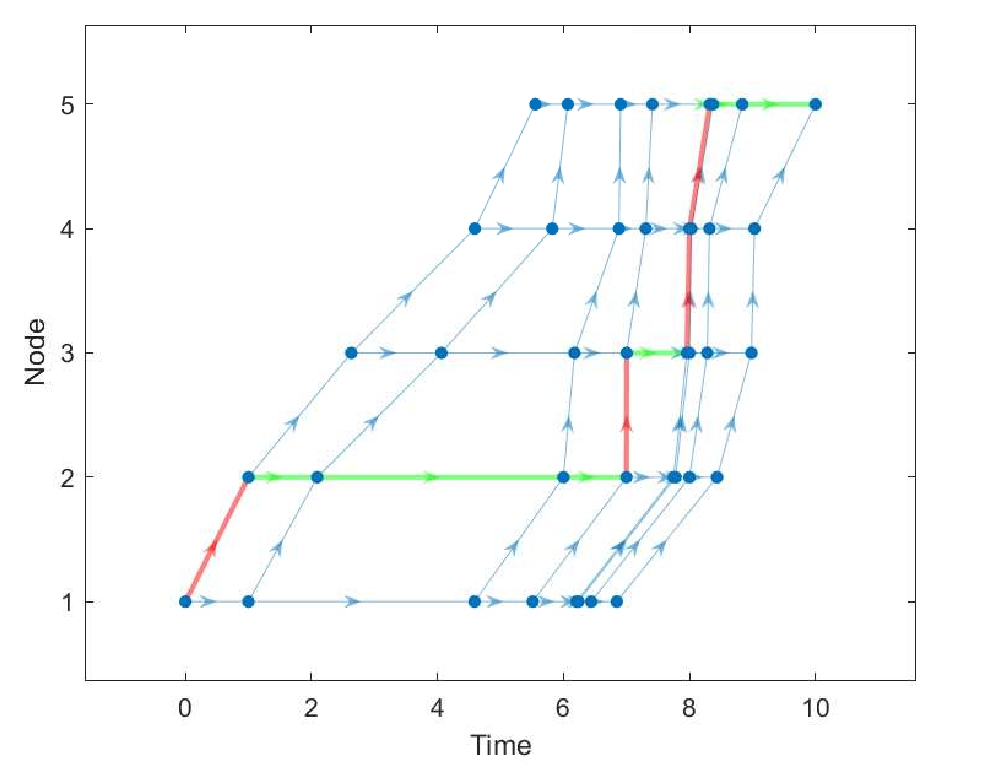
\includegraphics{edited-images/Figure7.jpg}
% \caption{Illustration of a timed path with 3 periods of
% waiting in green and 3 travel subpaths in red, in the TEN for a network
% consisting only of the arcs (1, 2), (2, 3), (3, 4) and (4, 5).}
\caption{Minh họa cho một đường đi có ba khoảng thời gian chờ đợi (màu xanh lá) và 
ba đường con (màu đỏ) với các cung \((1, 2), (2, 3), (3, 4)\)~và~\((4, 5)\) 
trong mạng TEN.}
\label{fig:7}
\end{figure}

\begin{definition}
\label{def:duong-di}
Trong một đường đi nhất định, \textbf{đoạn đường con} được tạo thành 
từ các nút con liên tiếp tối đa. Giả sử dãy nút đó
là \((i_1, t_1),...,(i_k, t_k)\), thỏa mãn hai điều kiện: 
\begin{enumerate}
  \item \(t_{l+1} =t_l + c_{i_l, i_{l+1}}(t_l)\) với mọi \(l = 1,\dots, k-2\), và
  \item \(t_k > t_{k-1} + c_{i_{k-1}, i_k}(t_k-1)\) (phải đợi tại nút
  \(i_k\)) hoặc \(t_k = t_{k-1} + c_{i_{k-1}, i_k}(t_k-1)\) với \(i_k=n\).
\end{enumerate}

\textbf{Đoạn đường con} được định nghĩa là dãy các nút
\((i_1, t_1),...,(i_{k-1}, t_{k-1}), (i_k, \tau)\), trong đó
\(\tau = t_{k−1} + c_{i_{k−1},i_k}(t_{k−1})\)
\end{definition}

Xét ví dụ, cho một dãy đường đi như sau:
\[((1,0);(2,6.9);(3,7.9);(4,8.1);(5,8.5))\] với \(\tau_{12} = 1\) ,
\(\tau_{23} = 0.2\), \(\tau_{34} = 0.2\) và \(\tau_{45} = 0.4\). Theo
\autoref{def:duong-di}, có ta đường con như sau: \[\{(1, 0); (2, 1)\}, \{(2, 6.9); (3, 7.1)\} \text{ và } \{(3, 7.9); (4, 8.1); (5, 8.5)\}\] 

\autoref{fig:7} minh hoạ cho ví dụ trên: Mạng TEN với
\[D = (\{1, 2, 3, 4, 5\}, \{(1, 2), (2, 3), (3, 4), (4, 5)\})\] 
Đường đi hiển thị bằng màu đỏ và xanh lá cây. 
Ba đoạn đường con của nó được tô màu đỏ.

Đường con là một phần của đường đi nhưng không có chờ đợi. Nó có các đặc
điểm như sau:

\begin{itemize}
\tightlist
\item
  Một đường con \textbf{\emph{không thể mở rộng ở hai đầu}} mà vẫn duy
  trì trạng thái không chờ đợi, hay:

  \begin{itemize}
  \tightlist
  \item
    Nếu hai nút \((i, t_i)\) và \((j, t_j)\) với \(i, j\) liên tiếp và
    \(t_j > t_i+c_{i,j}(t_i)\) thì nút \((j,t_i + c_{i,j}(t_i))\) là kết
    của đoạn con này và \((j, t_j)\) là nút đầu của đoạn con tiếp theo.
  \end{itemize}
\item
  Một đường đi có thể được tạo thành từ một tập các đường con, với thời
  gian chờ đợi xen giữa chúng.
\end{itemize}

Ví dụ: hình dung một người lái xe đi trên đường. Khi đi trên đường cao
tốc (đoạn đường con), người lái xe không cần dừng lại. Tuy nhiên, khi
đến ngã tư (điểm dừng), người lái xe phải dừng lại và chờ đèn giao
thông.

\begin{lemma}
\label{lem:toi-uu}
Cho một đường đi tối ưu
\(P\) của bài toán \(MTTP\) trên mạng \(D\) với hàm thời gian di chuyển
\(c\) và khoảng thời gian \([0,T]\). Xét một~\textbf{đường đi con}~\(S\)
bất kỳ của \(P\). Giả sử \(S\) bắt đầu tại nút \((i,t_i)\) và kết thúc
tại nút \((j,t_j)\). Khi đó \(S\) là nghiệm tối ưu cho bài toán
\textbf{MDP} trên cùng mạng \(D\), với cùng hàm \(c\), nhưng từ nguồn
\(i\) đến đích \(j\) và khoảng thời gian \([\tau^−,\tau^+]\), trong đó:
\(\tau^− \le t_i\) là thời gian kết thúc của \textbf{đường đi con}~ngay
trước \(S\) và \(\tau^+ \ge t_j\) là thời gian bắt đầu của đường đi
con~ngay sau S trong P (nếu có). Lưu ý rằng \(\tau^− = 0\) nếu \(i = 1\)
(không có đường đi con~nào trước \(S\)) và \(\tau^+ = T\) nếu \(j = n\)
(tức là không có~đường đi con~nào sau S).
\end{lemma}

\begin{proof}
\end{proof}

\begin{proposition}
\label{prp:mttp-toi-uu}
Với bất kỳ bài toán MTTP nào, đều có
một~\textbf{đường đi tối ưu}~sao cho mỗi~\textbf{đường con}~của nó đi
qua ít nhất một nút tại điểm dừng của hàm thời gian di chuyển.
\end{proposition}

\begin{proof}
\end{proof}

\begin{definition}
Một MTTP với các hàm thời gian di chuyển \(c\),
việc xây dựng mạng thời gian có độ dài của cung, gọi tắt là
\textbf{TENL}, như sau:

\begin{enumerate}
\def\labelenumi{\arabic{enumi}.}
\tightlist
\item
  Đối với mỗi~\textbf{điểm dừng}~\((i, t)\), giải hai bài toán con
  \textbf{TDSPP}: \(i-FSPT\) (kí hiệu \(\mathcal F^{i,t}\)) và \(i-BSPT\)
  (kí hiệu \(\mathcal B^{i,t}\)). Tạo ra TEN từ hợp của
  \(\mathcal F^{i,t}\) và \(\mathcal B^{i,t}\) với mọi \textbf{điểm
  dừng} có trong đó.
\item
  Đối với mỗi nút trong mạng TEN mới tạo, thêm các cung chờ đợi giữa các
  nút liền kề theo thứ tự thời gian.
\item
  Gán cho mọi cung, chẳng hạn như \(((i, t), (j, t' ))\), độ dài bằng \(0\) nếu \(j = i\) và độ
  dài bằng \(c_{i,j} (t)\) (và phải bằng \(t' − t\)).
\end{enumerate}

\end{definition}

Các nút \(1, 0\) và \(n, T\) là hai BP trong MTTP có các đỉnh \(\{1,\cdots, n\}\) 
với khung thời gian \([0,T]\), nên cũng là hai nút trong \textbf{TENL}.

\begin{corollary}
\label{col:mttp}
Cho một \textbf{MTTP} có tập các đỉnh
\(\{1,...,n\}\) với khung thời gian \([0,T]\), \textbf{bất kỳ}~đường
đi~ngắn nhất nào từ \((1,0)\) đến \((n,T)\) trong \textbf{TENL} đều
tương ứng là một nghiệm của bài toán \textbf{MTTP}.
\end{corollary}

\begin{proof} \end{proof}

\begin{proposition}
\label{prp:dpt-mttp}
Độ phức tạp cho \textbf{MTTP} trên đồ thị
có hướng \((N,A)\) với \(n = |N|\) đỉnh và \(K^{nodes}\) điểm dừng là
\[ (\mathcal{K}^{nodes} ×SSP(n,|A|)+ASPP(K^{nodes}n,K^{nodes}n)), \]
trong đó \(SPP(\alpha,\beta)\) là độ phức tạp của việc giải bài toán
\textbf{đường đi} ngắn nhất tĩnh trên đồ thị có hướng với \(\alpha\) nút
và \(\beta\) cung, và \(ASPP(\alpha,\beta)\) cũng tương tự nhưng đối với
một đồ thị có hướng phi chu trình.
\end{proposition}

\begin{proof} \end{proof}

\section{Công thức chi tiết}\label{cong-thuc2}

Trước khi đi vào chi tiết, hãy nhắc lại sự khác nhau của bài toán MDP và
MTTP: MDP sử dụng ABSPT để giảm số điểm dừng cần xử lý; trong khi MTTP
có cách tiếp cận khác. Theo Proposition 3.3, cấu trúc của ABSPT không
phù hợp với MTTP. Một nghiệm tối ưu cho MTTP là một chuỗi các đường đi
con được nối với nhau bằng cung chờ đợi; mỗi đường đi con được giả định
là đi qua một điểm gãy và thời gian chờ đợi luôn dương (\(>0\)).

\begin{definition}
\label{def:duong-di-con}
Một đường đi con qua điểm
dừng \((i, t)\), là một đường đi không chờ đợi nối một TDSP kết thúc tại
\((i, t)\) với một TDSP khác xuất phát từ \((i, t)\). Thuật ngữ
\textbf{đường đi con} sẽ không chỉ định điểm dừng, trong khi
\textbf{đường đi con \(i\)} được dùng để chỉ điểm dừng tại đỉnh \(i\)
vào thời điểm không xác định.
\end{definition}

Qua định nghĩa, luôn tồn tại một số~nghiệm~tối ưu cho MTTP mà
mỗi~\textbf{đường đi con}~của nó nằm trong một \textbf{TEN} được hình
thành bởi hợp FSPT và BSPT tại một~\textbf{điểm dừng}~xác định. Do đó,
thay vì dùng ABSPT, cấu trúc phù hợp hơn sử dụng để giải cho MTTP là hợp
của \(i-FSPT\) và \(i-BSPT\) cho cùng một điểm dừng tại đỉnh \(i\), gọi
là \(mangrove\). Lưu ý toán tử hợp (\(\cup\)) cũng được dùng để tạo một
TEN dưới dạng hợp của hai TEN.

\begin{definition}
\label{def:mangrove}
Một \(mangrove\) cho điểm dừng \((i, t)\), ký
hiệu là \(\mathcal M ^{i,t}\), là một TEN được tạo bằng cách lấy hợp của
\(\mathcal F^{i,t}\) và \(\mathcal B ^{i,t}\), hay
\(\mathcal M ^{i,t} = \mathcal F ^{i,t} \cup \mathcal B ^{i,t}\). Tôi gọi bất kì
\(mangrove\) nào như vậy là~\(i-mangrove\)~và sử dụng
\((i, t)-mangrove\) nếu chúng tôi muốn chỉ định cho điểm dừng
\((i, t)\).
\end{definition}

Giống với khi tính toán BSPT cho MDP, tính chất FIFO phải được đảm bảo
cho bất kì đỉnh \(i\) nào. Tập tất cả các \(i-mangrove\) luôn được sắp
xếp theo thời gian đối với các nút trong \(i-FSPT\) và tương tự với
\(i-BSPT\) của chúng. Cụ thể, nếu \(\mathcal M^{i, t}=F^{i,t}\cup B^{i,t}\)
và \(\mathcal M^{i, t'}=F^{i,t'}\cup B^{i,t'}\) với \((t’ > t\)), thì với
bất kì nút \(j\) nào có \((j,s) \in \mathcal F^{i, t}\) và
\((j,s’) \in \mathcal F^{i, t’}\) thì \(s’ > s\). Tương tự với các nút trong
\(i-BSPT\).

Do đó, bất kỳ đường đi con i nào đến đỉnh \(i\) tại thời gian \(t\) hoặc
muộn tạo thành nút \((i,t)\) hơn đều nằm trong một dãy các nút thuộc
\(\mathcal M^{i, t}\). Đương nhiên điều kiện là phải có các cung nối giữa
chúng. Đối với điểm gãy \((i, t)\) đã cho, cây AFSPT (kí hiệu
\(\mathcal{\overline{F}}^{i,t}\)) được tạo từ \(\mathcal F^{i,t}\) sau khi thêm
các cung \(((j, t'), (k, t''))\) chưa tồn tại, sao cho
\(\forall (j, k) \in A\) thì cả \((j,t')\) và \((k,t'')\) đều nằm trong
\(FSPT.\) Tương tự ta có định nghĩa của ABSPT như đã đề cập ở chương về
MDP. \(Mangrove\) hoàn chỉnh cho điểm dừng \((i, t)\), kí hiệu
(\(\overline{\mathcal M}^{i,t}\)) và là một TEN được tạo ra từ hợp của
\(\mathcal{\overline{F}}^{i,t}\) và \(\mathcal{\overline{B}}^{i,t}\).

Thuật toán được thực hiện bằng cách duy trì một tập các TEN, mỗi TEN là
một \(mangrove\) hoặc \(mangrove\) hoàn chỉnh cho một số điểm dừng. Mỗi
tập TEN con có chung đỉnh này được sắp xếp theo thời gian của các điểm
dừng. Với mỗi đỉnh \(i\) tương ứng có một danh sách \(L^i\) chứa các
điểm dừng \((i, t)\) sắp xếp theo thời gian. Với mỗi \((i, t)\) được
thêm vào \(L^i\) thì sẽ tính toán \(M^{i, t}\) và
\(\overline{\mathcal M}^{i,t}\). Với mỗi điểm dừng liên tiếp trong \(L^i\),
ví dụ như \((i,t)\) và \((i,t^+)\) với \(t^+ > t\), ta tiến hành như
sau:

\begin{itemize}
\tightlist
\item[i.]
  Trường hợp giữa \(t\) và \(t^+\) không có điểm dừng: \\
  Ta nói
  \(mangrove\) cho \((i, t)\) đã được giải quyết. Đặt UTT thành thời
  gian di chuyển thực tế:
  \[\underline c_{(i, s), (k, s')}:=c_{j, k}(s)\] với mỗi cung
  \(((j,s),(k,s’))\) trong \(\mathcal M^{i,t}\).
\item[ii.]
  Trường hợp còn lại khi \(mangrove\) cho \((i, t)\) chưa được giải
  quyết: \\
  Thuật toán đặt UTT trên mỗi cung \(((j, s), (k, s’))\) trong
  \(\mathcal M^{i,t}\)
  \[\underline c_{(i, s), (k, s')}:=\min_\tau\{c_{i, k}(\tau):s\le \tau \le s^+\}\]
  với \(s^+\) là thời gian duy nhất để nút \((j, s^+)\) nằm trong
  \(\mathcal{\overline{F}}^{i,t}\) (tương tự với \(\mathcal{\overline{B}}^{i,t}\)).
  Lúc này, bất kỳ đường con tại \(i\) trong khoảng thời gian \([t,t^+]\)
  xuất hiện trong đường đi của \(\overline{\mathcal M}^{i,t}\) thì đều có
  tổng UTT không lớn hơn thời gian di chuyển của đường đi đó.
\end{itemize}

Để đảm bảo rằng \(L^i\) luôn chứa các điểm dừng \emph{đủ sớm} với mọi
đỉnh \(i\), bất kì đường con nào cũng được biểu diễn bởi một đường đi
trong \(mangrove\) hoặc \(mangrove\) hoàn chỉnh với \(UTT\) là cận dưới
của thời gian di chuyển. Không mất tính tổng quát, thuật toán khởi tạo
\(L^i\) với điểm dừng \((i, 0)\) cho mỗi \(i\). (Trong thực nghiệm, việc
dùng \((i, t)\) với \(t\) là thời điểm ngay sau \(s\) nếu \((i, s)\)
thuộc \(\mathcal F^{1,0}\) sẽ hiệu quả hơn). Theo cách tương tự, tôi thêm
\((i, T)\) vào \(L^i\) và coi \((i, T)-mangrove\) được giải quyết và UTT
cho các cung là thời gian di chuyển thực tế.

Các \(i-mangrove\) cho các \(i\) khác nhau phải được kết nối bằng các
cung chờ đợi tại một nút nằm giữa các đường con.

Nhắc lại, thuật toán sẽ duy trì một TEN có kí hiệu \(\mathcal D_{LB}\),
với các UTT liên quan trên mỗi cung, và được định nghĩa là một hàm của
các \(mangrove\) và \(mangrove\) hoàn chỉnh có các điểm dừng thuộc tập
\(\bigcup _{i\in N} L^i\) như sau:

\underline{Các nút và các cung:} Tất cả các nút và cung trong \(mangrove\) được giải
quyết và \(mangrove\) hoàn chỉnh đều được đưa vào \(\mathcal D_{LB}\)
cùng với các UTT của chúng.

\underline{Cung chờ:} Các cung chờ được đưa vào để kết nối \(mangrove\) (hoàn
chỉnh)\footnote{Mangrove hoặc mangrove hoàn chỉnh đã được giải quyết.}
đại diện cho một đường con đến một mangrove (hoàn chỉnh) khác có thể đại
diện cho đường con kế tiếp. Có nghĩa là sẽ xem xét bất kỳ đường con
\(i\) nào kết thúc tại đỉnh \(j\), sau đó chờ tại \(j\), kế tiếp là
đường con \(k\) bắt đầu tại \(j\) (với \(k\neq i\)) trong khi đảm bảo
UTT của nó không lớn hơn thời gian thực tế. Ta chỉ xét thời gian chờ
dương tại \(j\).


% \begin{figure}
%     \centering
%     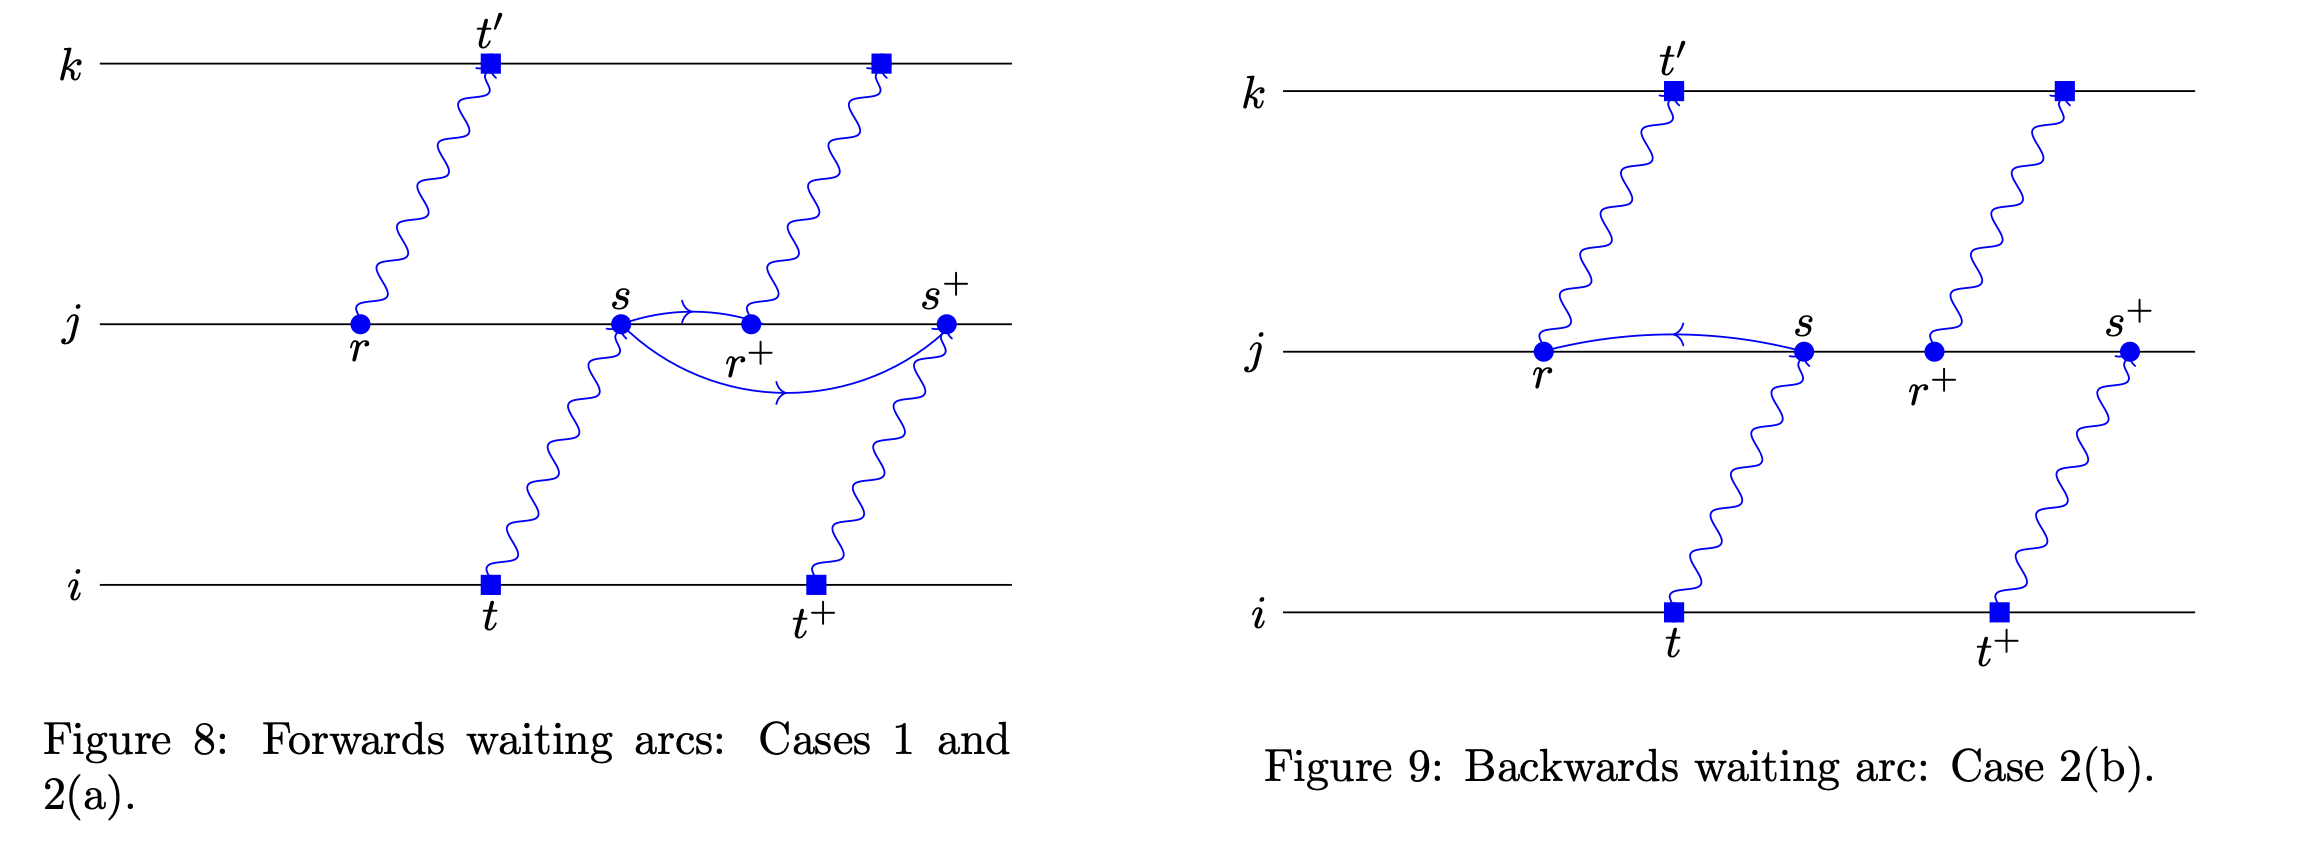
\includegraphics{images/Figure8_9.png} 
%     \caption{Hình vuông nhỏ kí hiệu cho ``gốc'' của \(mangrove\), hình
% tròn biểu diễn cho một nút và đường con được biểu diễn bởi đường xoắn
% màu xanh biển.}
%     \label{fig:8_9}
% \end{figure}
\begin{figure}[H]
    \centering
    \captionbox{Cung chờ tiến: TH1 và TH2(a)\label{fig:8}}{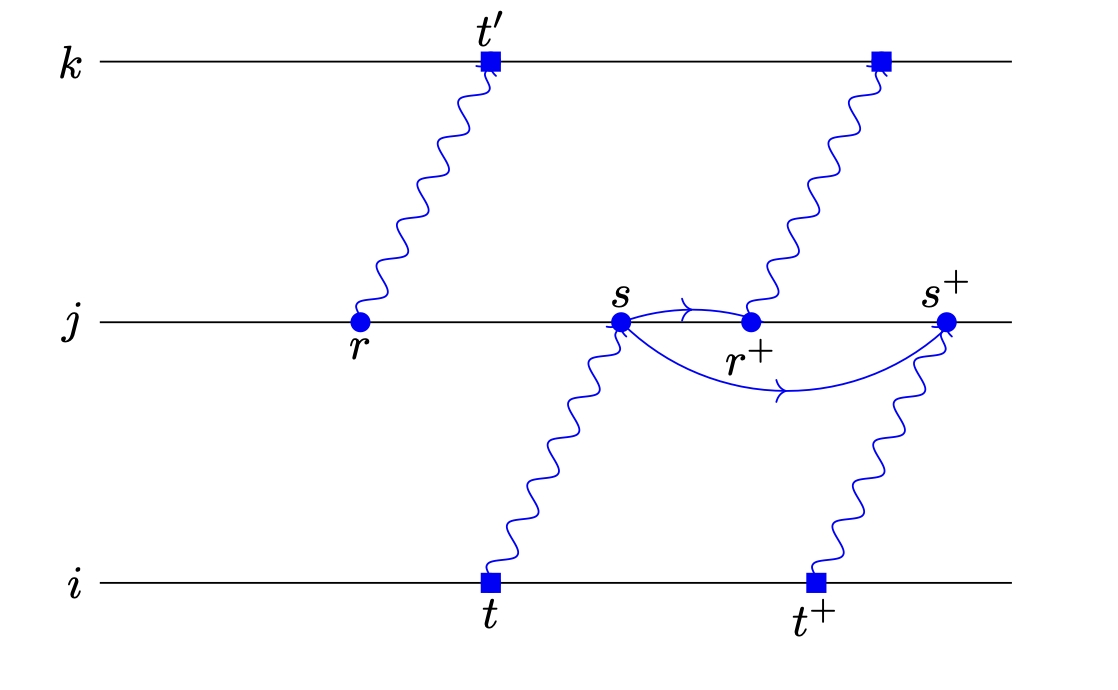
\includegraphics[width=0.45\linewidth]{edited-images/Figure8.jpg}}
    \captionbox{Cung chờ lùi: TH2(b)\label{fig:9}}{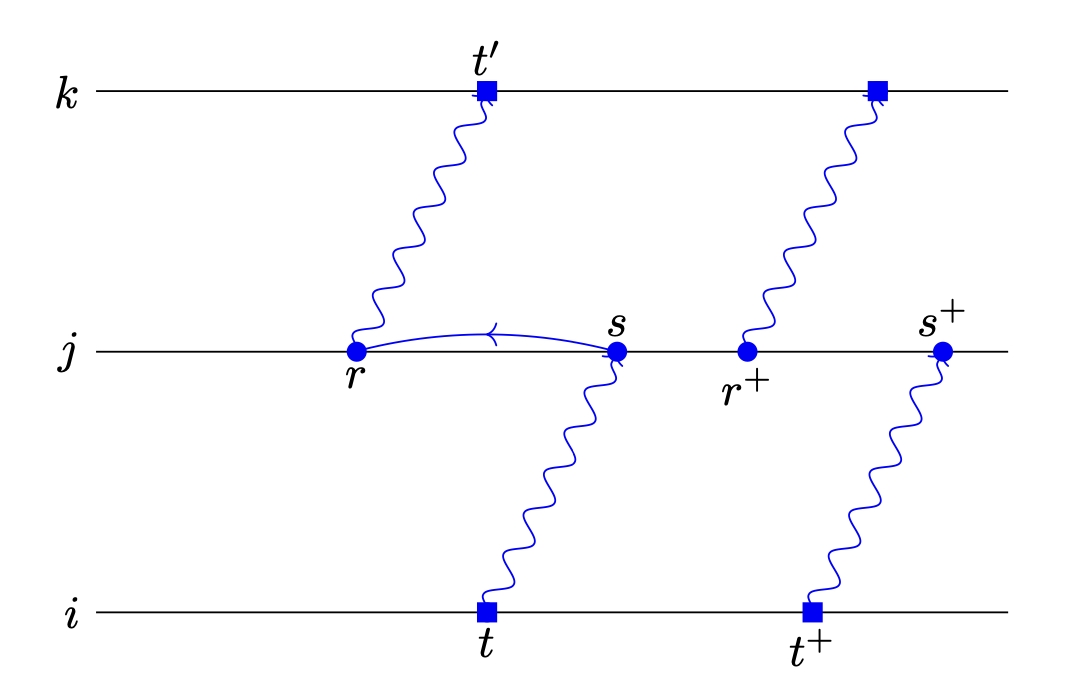
\includegraphics[width=0.45\linewidth]{edited-images/Figure9.jpg}}
    \\
    Giải thích \\

    \flushleft

    \begin{tabular}{lc}
      hình vuông: & gốc của \(mangrove\),\\ 
      hình tròn: & nút, \\
      dây xoắn: & đường con.      
    \end{tabular}
\end{figure}

Các trường hợp có thể xảy ra như sau:

\begin{enumerate}
\def\labelenumi{\arabic{enumi}.}
\item[\textbf{TH1:}]
Để biểu diễn cung chờ tại đỉnh \(j\) đến thời
  điểm \(s^+\) hoặc muộn hơn, ta thêm cung \(((j, s), (j, s^+))\) vào
  \(\mathcal D_{LB}\) và gán UTT bằng \(0\). Các cung chờ nối các nút có
  trong các BSPT cho \(mangrove-i\) liên tiếp thuộc \(L^i\) là không cần
  thiết nên ta có thể giả sử rằng việc chờ đợi chỉ xảy ra ở cuối một
  đường con chứ không phải ở đầu (không mất tính tổng quát).
\item[\textbf{TH2:}]
   Đối với mỗi đỉnh \(k\neq i\), lấy \(r\) là thời
  điểm ngay trước \(s\) sao cho nút \((j,r)\) xuất hiện trong BSPT cho
  một \(mangrove-k\), giả sử là \(\mathcal M^{k,t'}\). (Cách chọn này sẽ
  không tồn tại \(t'' > t'\) với \(\mathcal M^{k,t''}\) trong \(L^k\) có
  chứa \((j,r')\) trong \(\mathcal B^{k,t''}\) với \(r < r' < s\).) Chắc
  chắn phải tồn tại \(t'\) và \(r\) như vậy, vì \((j, s)\) trong
  \(\mathcal F^{i,t}\) đồng nghĩa với việc hoặc \(s>0\), hoặc \(i = j\) và
  \(s = t = 0\), trong khi bất kì nút nào trong \(\mathcal B^{k,0}\) đều có
  thời gian âm ngoại trừ ở \(k\) và tôi đã khởi tại \(L^k\) với
  \((k,0)\) nằm trong. Ngoài ra, nếu \(t'<T\), lấy \(r^+\) sao cho
  \((j,r^+)\) nằm trong BSPT cho \(mangrove\) có điểm dừng tiếp theo
  trong \(L^k\) sau \((k, t')\). Lưu ý \(r^+ \geq s\). Xét hai trường
  hợp phụ sau:

  \begin{enumerate}
  \def\labelenumii{\alph{enumii}.}
  \tightlist
  \item
    \(Mangrove\) cho \((k, t')\) đã được giải quyết: \\
    Không cần cung chờ
    nào nối \((j,s)\) với \(mangrove\) cho \((k,t')\) vì \(mangrove\)
    này chỉ biểu diễn các đường con \((k,t')\) và không thể đến được nút
    \((k, t')\) với thời gian chờ dương tại \((j, s)\). - Nếu \(t'=T\)
    thì không có \(k-mangrove\) tiếp theo sau \((k,t')-mangrove\). -
    Ngược lại, \((j,s)\) được nối với \(k-mangrove\) tiếp theo: thêm
    cung \(((j,s),(j,r^+))\) vào \(\mathcal D_{LB}\), với UTT bằng
    \(0\), điều này cho phép \(\mathcal D_{LB}\) biểu diễn chuỗi của:
    đường con \(i\) kết thúc tại \(j\) ở thời điểm \(r\in [s,s^+)\),
    đường con \(k\) bắt đầu tại \(j\) ở thời điểm \(\tau \in [s, s^+)\),
    và đường con \(k\) bắt đầu tại \(j\) ở thời điểm \(\tau' > \tau\),
    sử dụng điểm dừng tiếp theo tại \(k\) sau \(t'\). Vì \(r^+ \geq s\)
    nên gọi \(((j,s),(j,r^+))\) là \textbf{cung chờ tiến.}
  \item
    \(Mangrove\) cho \((k, t')\) chưa được giải quyết: \\
    Cung
    \(((j,s),(j,r))\) được đưa vào \(\mathcal D_{LB}\) với UTT bằng 0.
    Lúc này, \(\mathcal D_{LB}\) có thể biểu diễn chuỗi của một đường
    con \(i\) kết thúc tại \(j\) ở thời điểm \(\tau \in [s,s+)\) và
    đường con \(k\) bắt đầu tại \(j\) ở thời điểm
    \(\tau' \in [\tau,r^+)\). Vì \(r\leq s\) nên gọi \(((j,s),(j,r))\)
    là \textbf{cung chờ lùi.}
  \end{enumerate}
\end{enumerate}



\begin{figure}
\centering
% 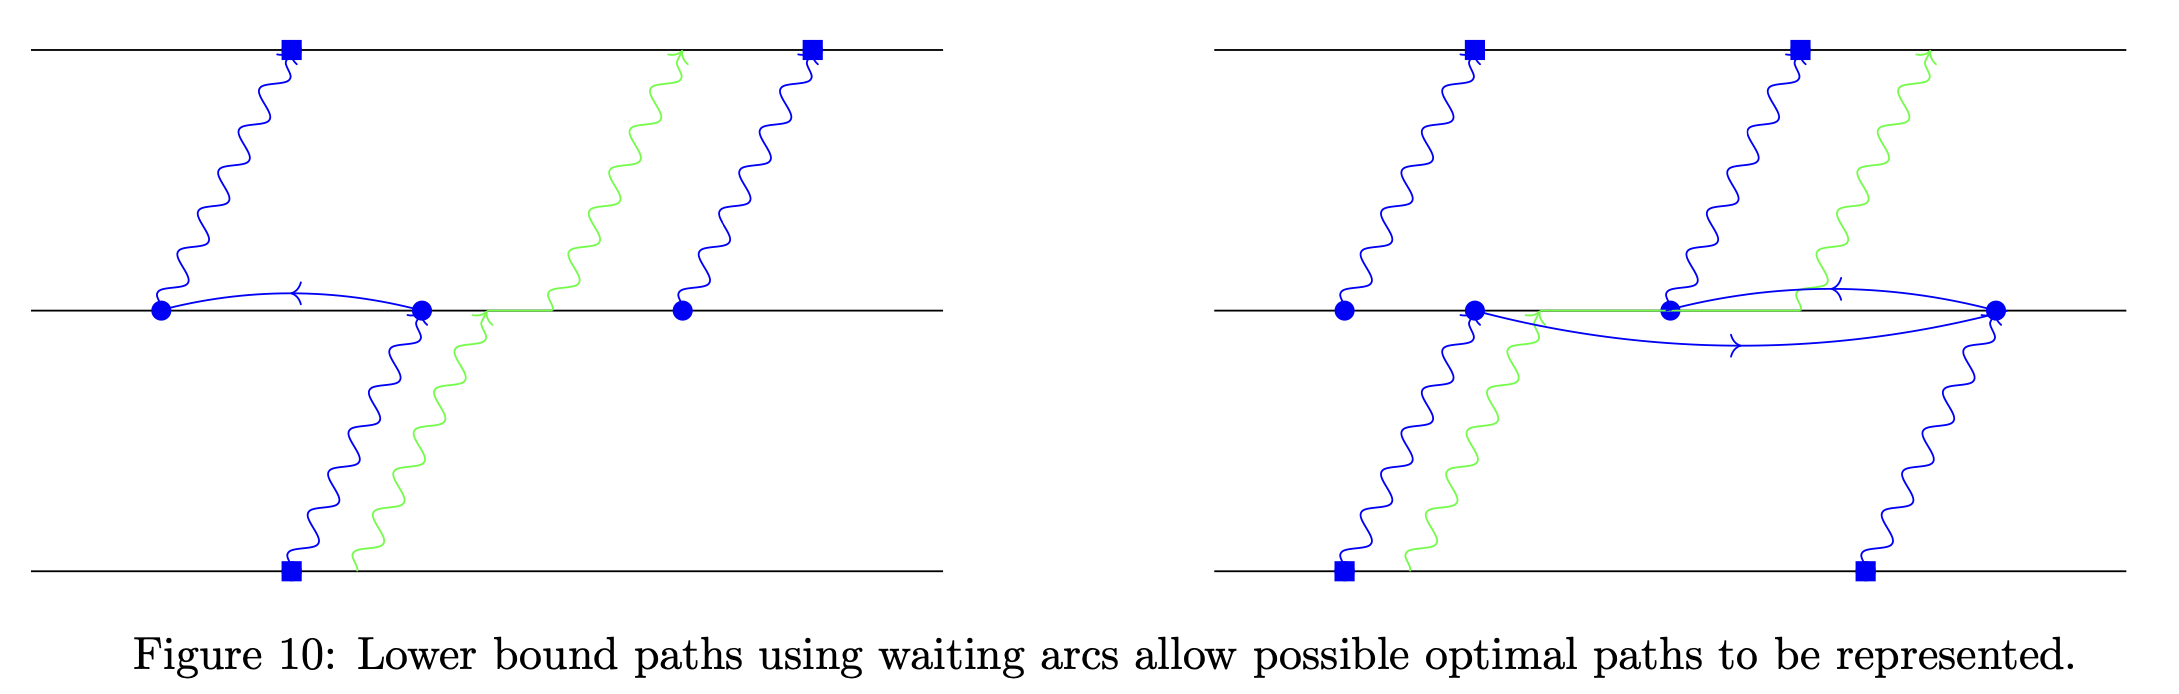
\includegraphics{images/Figure10.png}
\subcaptionbox*{}{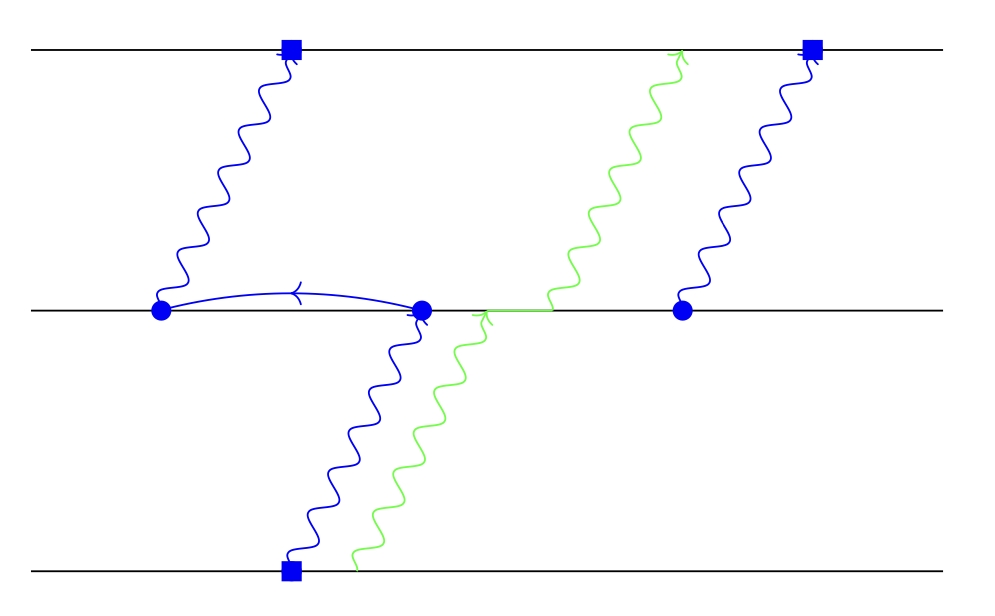
\includegraphics[width=0.45\linewidth]{edited-images/Figure10a.jpg}}
\subcaptionbox*{}{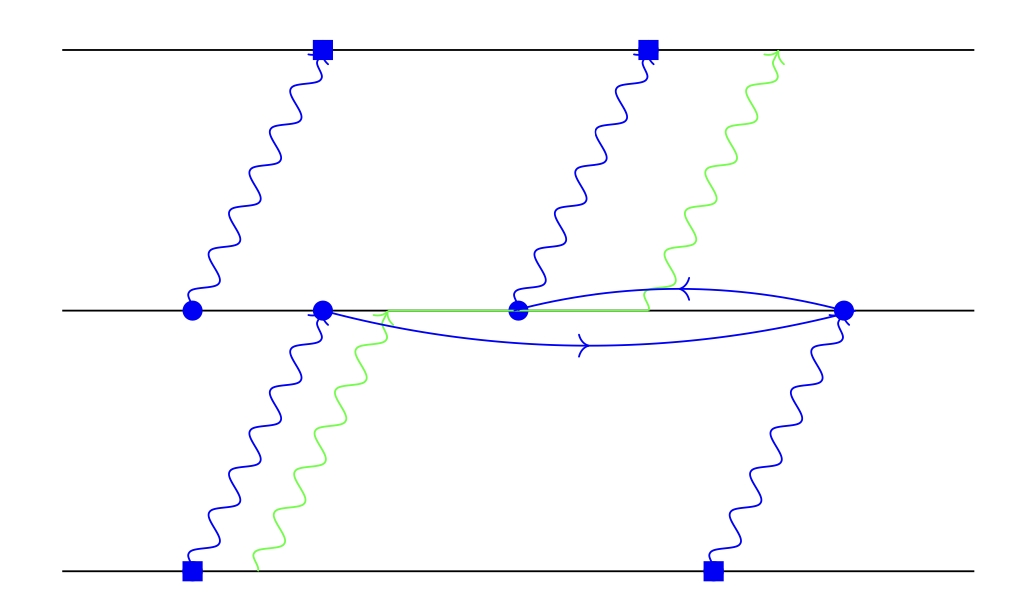
\includegraphics[width=0.45\linewidth]{edited-images/Figure10b.jpg}}
\caption{Cách các cung chờ giúp TEN tìm được các đường đi tối ưu
(màu xanh lá cây)}
\label{fig:10}
\end{figure}

\underline{Các nút và cung ảo:} Thêm một nút bắt đầu ảo và một nút kết thúc ảo vào
\(\mathcal D_{LB}\). Thêm các cung nối nút bắt đầu ảo với các nút có
dạng \((1,t)\) với \(t\geq 0\) và các nút có dạng \((n,t)\) với
\(t\leq T\) nối với nút kết thúc ảo. Tất cả các cung thêm vào đều có UTT
bằng \(0\).

Đường đi có UTT nhỏ nhất trong \(\mathcal D_{LB}\) được xây dựng như
trên, tính từ nút bắt đầu ảo đến nút kết thúc ảo, giá trị UTT sẽ là cận
dưới cho bài toán MTTP. Điều này được giải thích dưới đây.

Xét một nghiệm tối ưu trong MTTP, gồm hai đoạn con:

\begin{itemize}
\tightlist
\item

  Đoạn con \((i,\alpha)\) \(P_1^*\): Di chuyển từ nút \((i, \alpha)\)
  đến \((j, \alpha')\) mà không chờ đợi.
\item
  Đoạn con \((k,\beta')\) \(P_2^*\): Di chuyển từ nút \((j,\beta)\) đến
  \((k,\beta')\), với \(\beta -  \alpha' > 0\) là thời gian chờ đợi tại
  điểm \(j\).
\end{itemize}

Gọi \((i, s)\) là điểm cuối của danh sách \(L^i\) với \(s \leq \alpha\)
và \((k,t')\) là điểm cuối của \(L^k\) với \(t' \leq \beta'\). Lúc này
\(P_1^*\) là đường đi trong \(\overline{\mathcal M}^{i,s}\) với UTT cận trên
là thời gian di chuyển của \(P_1^*\) và tương tự với \(P_2^*\) cho
\(\overline{\mathcal M}^{k,t'}\). Từ \(\mathcal{\overline{F}}^{i,s}\) cho ra duy
nhất nút \((j, s')\) và \(\mathcal{\overline{B}}^{k,t'}\) cho ra duy nhất nút
\((j,t)\) đỉnh \(j\). Luôn có một đường đi trong \(\mathcal D_{LB}\) từ
\((j, s')\) đến \((j,t)\) với UTT bằng \(0\), theo như cách xây dựng ở
trên. Quan sát rằng \(s'\leq \alpha\) và \(t\leq \beta\) bởi thứ tự đã
được sắp xếp của các \(mangrove\) cho cùng đỉnh.

Tuy nhiên \(t-s'\) có thể âm:

\begin{itemize}
\tightlist
\item
  Nếu \(t<s'\) thì \((k,t')-mangrove\) không thể giải (vì nếu ngược lại,
  bắt buộc \(t'=\beta'\) và \(t=\beta>\alpha'\geq s'\)), vậy nên cung
  chờ lùi \(((j,t),(j,s'))\) được thêm vào \(\mathcal D_{LB}\) như trong
  Trường hợp 2(b).
\item
  Nếu \(t\geq s'\), có 2 trường hợp con như sau:

  \begin{itemize}
  \tightlist
  \item
    \((k,t')-mangrove\) giải được, cung chờ tiến \(((j,t),(j,s'))\) được
    thêm vào \(\mathcal D_{LB}\) như trong Trường hợp 2(a),
  \item
    Ngược lại, gọi \((i,r)\) là điểm đầu tiên ngay sau \((i,s)\) trong
    danh sách \(L^i\) sao cho điểm duy nhất \((j,r')\) từ
    \(\mathcal F^{i,r}\) có \(r' \geq t\). (\(r\) luôn tồn tại vì
    \(j\neq n\) và \((i,T)\) thuộc \(L^i\)). Lúc này:

    \begin{itemize}
    \tightlist
    \item
      Theo Trường hợp 1, sẽ có một chuỗi các cung có UTT\(=0\) nối
      \((j,s')\) với \((j,r')\), và
    \item
      Theo Trường hợp 2(b), sẽ có cung chờ lùi \(((j, r'), (j, s'))\) có
      UTT \(=0\) trong \(\mathcal D_{LB}\).
    \end{itemize}
  \end{itemize}
\end{itemize}

\textbf{Kết luận:} Trong mọi trường hợp, luôn có một đường đi UTT bằng 0 trong
\((j, t)\) đi từ \((j, s')\) đến \((j, t)\). Do đó, đoạn con \(P_1^*\)
nối tiếp \(P_2^*\) được biểu diễn trong \(\mathcal D_{LB}\) với một
đường đi có UTT không lớn hơn tổng thời gian di chuyển của \(P_1^*\) và
\(P_2^*\).

\section{Mô tả thuật toán}\label{muxf4-tux1ea3-thuux1eadt-touxe1n}

\begin{proposition}
Sử dụng quy trình ở trên, chúng ta có thể xây dựng
\(\mathcal D_{LB}\) và \(UTT\) cho mỗi cung trong \(\mathcal D_{LB}\) từ
các danh sách \(L^i\) có các nút \((i,0),(i,T) \in L^i\) với mỗi đỉnh
\(i \in N\). Sau đó, đường đi \(UTT\) ngắn nhất trong
\(\mathcal D_{LB}\) từ nút bắt đầu ảo đến nút kết thúc ảo có \(UTT\)
là~\textbf{cận dưới}~của MTTP.
\end{proposition}

Thuật toán sử dụng hai hàm như sau:

\begin{itemize}
\tightlist
\item
  \(createLBTEN(\{L^i\}_{i\in N}, Resolved)\): Xây dựng
  \(\mathcal D_{LB}\) và các UTT tương ứng, được lưu lại trong
  vector~\(\underline{c}\)~(như đã mô tả ở trên).~\(Resolved\)~là tập
  hợp các điểm mốc đã được giải quyết.
\item
  \(computeSP(\mathcal D_{LB},c)\): Tính toán đường đi có UTT nhỏ nhất
  trong \(\mathcal D_{LB}\), trả về cả đường đi và tổng UTT của nó.
\end{itemize}

Thêm vào đó, các danh sách \(\{L^i\}_{i\in N}\) cũng được dùng để tạo ra
\textbf{cận trên} bằng cách xây dựng một mạng TEN kí hiệu là
\(\mathcal D_{UB}\) theo các bước như sau:

\begin{enumerate}
\def\labelenumi{\arabic{enumi}.}
\tightlist
\item
  Tất cả các cung thuộc \((i,t)-mangrove\) với \((i,t)\) thuộc \(L^i\)
  và tất cả \(i\in N\) đều cho vào \(\mathcal D_{UB}\), với thời gian di
  chuyển ban đầu.
\item
  Với mỗi \((j,s)\) trong FSPT của một \(i-mangrove\) nào đó và với mỗi
  \(k\neq i\), tìm \(r\) là thời điểm ngay sau \(s\) mà nút \((j,r)\)
  xuất hiện trong BSPT của một \(k-mangrove\) (nếu có). Nếu tìm được
  \(r\) thoả mãn, thêm cung đợi \(((j, s), (j, r))\) vào
  \(\mathcal D_{UB}\) và đặt thời gian di chuyển là \(0\).
\item
  Thêm một nút bắt đầu ảo và kết thúc ảo vào \(\mathcal D_{UB}\). Thêm
  các cung để nối nút bắt đầu ảo với các nút có dạng \((1,t)\) với
  \(t\geq 0\), tương tự với các nút có dạng \((n,t)\) với \(t\leq T\)
  nối đến nút kết thúc ảo. Tất cả cung được thêm vào đều có thời gian di
  chuyển là \(0\).
\end{enumerate}

Bất kì đường đi nào trong mạng \(\mathcal D_{UB}\), từ nút bắt đầu ảo
đến kết thúc ảo, đều là một nghiệm khả thi, và tổng thời gian di chuyển
tạo ra \textbf{cận trên} cho bài toán MTTP. Bằng cách tối thiểu hoá thời
gian di chuyển, ta sẽ dần tìm ra cận trên tốt hơn từ
\(\mathcal D_{UB}\).

Thuật toán sẽ sử dụng hai hàm dưới đây để tạo ra mạng
\(\mathcal D_{UB}\):

\begin{itemize}
\tightlist
\item
  \(createUBTEN(\{L^i\}_{i\in N})\): Xây dựng mạng \(\mathcal D_{UB}\),
  và lưu lại các thời gian di chuyển tương ứng trong
  vector~\(\overline{c}\)~(như đã mô tả ở trên).
\item
  \(computeSP(\mathcal D_{UB},\overline{c})\): Tìm đường đi khả thi tốt
  nhất ở hiện tại cho MTTP, trả về cả đường đi và tổng thời gian di
  chuyển của nó.
\end{itemize}

Sau khi có các công cụ cần thiết, ta tiến hành xây dựng thuật toán 2 cho
bài toán MTTP theo hai bước như sau:



\begin{itemize}
  \item[\textbf{B1.}] Khởi tạo: 
\end{itemize}  
\begin{easylist}[itemize]
    @ Xây dựng hai mạng: 
        @@ Mạng TEN \(\mathcal D_{LB}\), 
        @@ Mạng TEN \(\mathcal D_{UB}\). 
    @ Tìm cận trên và cận dưới cho thời gian di chuyển bằng cách tìm đường đi trên mỗi mạng.
\end{easylist}

\begin{itemize}  
\item[\textbf{B2.}] Lặp lại bước này cho đến khi 2 cận bằng nhau: 
\end{itemize}
\begin{easylist}[itemize]
    @ Nếu hai cận chưa bằng nhau: 
        @@ Xét đường đi có UTT nhỏ nhất trong \(\mathcal D_{LB}\) và \(mangrove\) hoàn chỉnh đã được dùng. 
        @@ Ít nhất một trong các \((i,t)-mangrove\) đã được dùng có điểm dừng \((i,t)\) chưa được giải quyết, nếu không thì cận trên và cận dưới đã bằng nhau. 
        @@ Thuật toán chọn ra một tập bao gồm một hay nhiều điểm dừng chưa giải quyết như vậy.
        @@ Đối với mỗi điểm dừng (giả sử là \((i,t)\)) trong tập đã chọn: 
            @@@ Chọn một số điểm dừng (một hoặc nhiều) giữa \((i,t)\) và điểm tiếp theo trong \(L^i\), 
            @@@ Thêm các điểm dừng đã chọn vào \(L^i\), 
            @@@ Nếu có bất kì nút nào trong \(L^i\) ngay sau điểm dừng \((i,s)\) cũng thuộc \(L^i\), ta coi \((i,s)\) đã được giải quyết. 
    @ Tiếp tục tạo các \(\mathcal D_{LB}\) và \(\mathcal D_{UB}\) dựa trên \(L^i\) đã cập nhật, sau đó tính toán lại các cận trên và dưới.
\end{easylist}

Hiệu năng của thuật toán này mấu chốt nằm ở hai vấn đề sau:

\begin{enumerate}
\def\labelenumi{\arabic{enumi}.}
\tightlist
\item
  \textbf{Tập điểm dừng chưa giải quyết:}~Trong mỗi lần lặp, thuật toán
  cần chọn một tập các điểm dừng~chưa được giải quyết,
\item
  \textbf{Tập điểm dừng cho cùng đỉnh:} Trong mỗi lần lặp, cần chọn tập
  điểm dừng có chung một đỉnh để đưa vào danh sách của đỉnh đó.
\end{enumerate}

Chi tiết về vấn đề này sẽ được đề cập ở \autoref{kux1ecbch-bux1ea3n-vuxe0-cuxe0i-ux111ux1eb7t}. 
Ở đây sẽ không đi vào chi tiết (để đơn giản hoá cho mã giả). Hàm \(FindBP(P, \{L^i\}_{i\in N})\) được dùng để xác định tập các BP
mới thêm vào danh sách \(L^i\), dựa trên đường đi có UTT nhỏ nhất
\(P\) tìm được từ \(\mathcal{D}_{LB}\). 

\section{Mã giả}

\begin{algorithm}[H]
\caption{Dynamic Discretization Discovery Algorithm for the MTTP}
\label{algo:2}
\begin{algorithmic}
    \Input{digraph $D = (N, A)$, latest time at end node $T$, arc travel time function $c_{i, j}(t)$ for all $t \in [0, T]$, for each $(i, j) \in A$}
    \Output{minimum travel time path from node $1$ to $n$ departing from $1$ and arriving at $n$ at times in $[0, T]$}
    
\State $Resolved := \emptyset;$

\For{$i \gets 1$ \To $n$}

    \State Compute the $(i, 0)$-mangrove and the arc-completed $(i, 0)$-mangrove; 
    \State Compute the $(i, T)$-mangrove and the arc-completed $(i, T)$-mangrove; 
    \State Set $L^i := [(i, 0), (i, T )]$ ;
    \State $Resolved := Resolved \cup {(i, T )}$;
\EndFor

\State Initialize $LB = −\infty$ and $UB = \infty$; 

\While{$(LB < UB)$}
    \State Construct lower and upper bound TENs, with their UTTs and travel times, respectively:
        \State  $(\mathcal{D}_{LB},\underline{c}) \gets createLBTEN(\{L^i\}_{i\in N},Resolved), \\(\mathcal{D}_{UB},\overline{c}) \gets createUBTEN(\{L^i\}_{i\in N})$ ;
    \State Compute current lower and upper bounds along with their corresponding path:
        \State  $(P_{LB},LB)\gets computeSP(D_{LB},\underline{c}),(P_{UB},UB) \gets computeSP(D_{UB},\overline{c})$ ;
    \State $BP \gets findBP(P_{LB},\{L^i\}_{i\in N}) ;$
    \For{$(j,t) \in BP$}
    \EndFor 
        \State Compute the $(j, t)$-mangrove and the arc-completed $(j, t)$-mangrove;
        \State Insert $(j,t)$ in the list $L^j$;
        \If{$(j,t^−)$ is in $L^j$ immediately before $(j,t)$ and no breakpoint at $j$ is between them}
        \State          $Resolved := Resolved \cup {(j, t−)}$
        \EndIf
        \If{$(j,t^+)$ is in $L^j$ immediately after $(j,t)$ and no breakpoint at $j$ is between them}
        \State  $Resolved := Resolved \cup {(j, t)}$ 

        \EndIf  
\EndWhile

\Return $(UB,P_{UB})$

    \end{algorithmic}
\end{algorithm}

\backmatter
\end{document}
% END DOCUMENT